\documentclass{article}


% *** *** *** %
\usepackage{indentfirst}
\usepackage{graphicx}
\usepackage{url}
\usepackage{tikz}
\usepackage{subfigure}
\def\tm{\leavevmode\hbox{$\rm {}^{TM}$}} %\tm
\newcommand{\cs}{C\slash S}
% *** *** *** %


\begin{document}

\title{Egal Car: A Synchronized Peer-to-Peer Car Racing Game Over Named Data Networking}
\author{Zening Qu}
\date{\today}
\maketitle

\begin{abstract}
Blahblahblah
\end{abstract}

%============================================================================%
\section{Introduction}
\label{introduction}

One of the most important differences between a multiplayer on-line game (MOG) and a single player game is that in the former case there exists a virtual world that needs to be shared and maintained \emph{consistent}. Consistency maintenance is about guaranteeing that all players in the shared virtual world will have correct understanding of it. For example, in a game that provides a global view to its players, everyone should be able to view the position of all other players in real time, and there should not be any collision between any two views. 

Synchronization mechanisms are fundamental to consistency maintenance. In a MOG where players are usually distributed in a wide geographic area, delivery of game state updates relies solely on the packets transmitted through the network. If the lower layers only provide connectionless services, which is highly possible since MOGs typically use IP and UDP, it can be imagined that those packet updates will be out of order when received by players. This is a potential hazard to MOGs because normally game state updates should be processed in the order of their generation time in order for players to learn the chronological and causal relationship between updates. If packets were not processed in the correct order, different players would have different understanding of the game state. In other words, \emph{inconsistency} would arise. A synchronization mechanism avoids inconsistency by making sure that all players process update packets in the correct order (see section~\ref{ndnbackground}). With a synchronization mechanism every copy of the game application receives consistent input from the network, therefore their outputs will be consistent, too.
\footnote{Note that game state consistency can also be achieved by using connection-oriented protocols such as TCP in the lower layers. However, research has shown that such protocols may result in severe performance degradation and thus are rarely used by MOGs~\cite{Fgame}.}

This paper documents a simple synchronization mechanism that we designed for MOGs over named data network (NDN)~\cite{Jndn}. NDN is a new Internet architecture that names data instead of hosts (see section~\ref{ndnbackground}). From the game application's point of view, NDN can be regarded as a new lower layer service provider, or an alternative of TCP\slash IP. But NDN's impact on game development and synchronization mechanism may go beyond that: as data acquire names that are meaningful to game applications, the method for managing and synchronizing these data evolves accordingly. % :)

We explored NDN's impact on MOG design and implementation by creating a MOG on our NDN testbed. Our game prototype is called \emph{Egal Car}, which is a 3D car racing game with highly detailed scenery and track. Each player has control over one car, which can speed up, slow down and alter direction. The cars can collide with each other and with fences along the track. All car movements are simulated by the game's physics engine. Like in any racing game, each player's goal is to lead the other competitors and win the race. Note that Egal Car is adapted from an open source game template called Unity\tm  Car Tutorial~\cite{UnityCar}. This template provides all graphics and physics modules that we mentioned above, but does not contain a network module. In other words, the template is a single-player off-line car racing game with all front-end work done; it only takes a network module to become a MOG. We designed and engineered the network module of this game. Specifically, we designed a synchronization mechanism with the car racing game's needs in mind. 

The rest of this paper describes the design choices and implementation details of our prototype game and its network module. Section~\ref{ndnbackground}~introduces NDN principles and facts that may inspire MOG design. Sections~\ref{architecture}~through~\ref{implementation}~discuss MOG design, using Egal Car as a main example.


%============================================================================%
\section{NDN Background}
\label{ndnbackground}

NDN differs from IP in that every piece of NDN data can have a \emph{name} that is meaningful to its consumer (the application who processes the data). To retrieve a piece of data, the receiver must know the data's name, but he/she does not have to know the data's location (host address) as in the IP network. NDN communication is established on the two packet types: \emph{Interest} and \emph{Data}. An Interest is a packet issued by the data receiver to express that a certain piece of data is needed. A Data is a packet published by the sender in response to an Interest. Both Interest and Data use names to identify the data being exchanged (see figure~\ref{img:packet_types}). An Interest is `satisfied' by a Data if its Content Name is a prefix of the Content Name in the Data packet.~\cite{Jndn}

\begin{figure}
\begin{center}
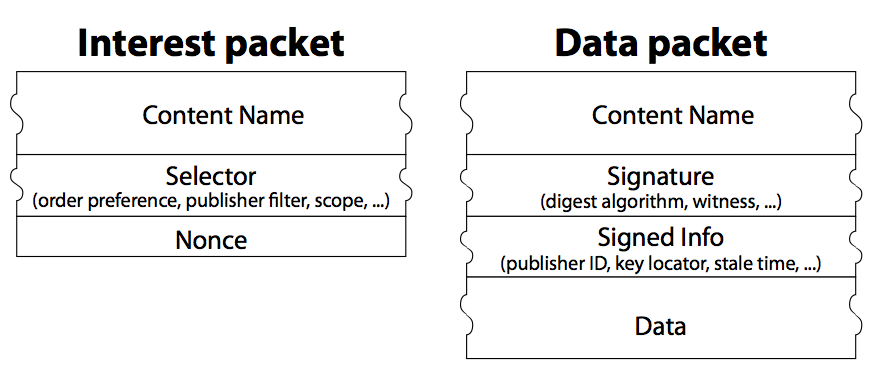
\includegraphics[width=0.7\textwidth] {image/packet_types}
\caption{Interest packet and Data packet}
\label{img:packet_types}
\end{center}
\end{figure}

% introduce CCNx and Sync
There are a few general purpose synchronization protocols under development. Among them is the CCNx Synchronization Protocol~\cite{CCNxSync} (CCNx Sync). CCNx\textregistered~is an implementation of NDN and open source project of PARC\textregistered. CCNx Sync is a facility provided by the CCNx project to help applications to maintain data integrity. It should be noted that, CCNx Sync, and other general purpose synchronization protocols are different from the game synchronization mechanisms that we mentioned in section~\ref{introduction}. The general purpose protocols maintain data integrity while the game protocols ensure game state consistency. Nevertheless, CCNx Sync can be utilized by MOGs in many situations. In fact, through our experiment we found that CCNx Sync brings lots of conveniences to MOG development. We demonstrate the use of CCNx Sync in Egal Car in section~\ref{synchronization}.


%============================================================================%
\section{Architecture}
\label{architecture}

When designing the network module of a MOG, the first decision that should be made is what architecture the MOG should use. Game architecture is a defining factor of the game's scalability, robustness and performance, and it has a fundamental influence on other game design choices such as the choice of synchronization mechanisms. As the network transmission strategy has changed in NDN, the preference of game architectures may also change.

There are two classes of game architectures, Client\slash Server (\cs) and Peer-to-Peer (P2P). In \cs~architectures all clients are directly connected to a central server which is the only authorized source of game state updates (see figure~\ref{cs}). In P2P architectures, peers (clients) are inter-connected and each peer computes newer game state on its own (see figure~\ref{p2p}). 

\begin{figure} 
\centering  
\subfigure[\cs]  
{  
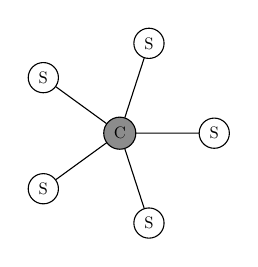
\begin{tikzpicture} [scale=0.6, transform shape]
\tikzstyle{every node}=[draw,shape=circle];
\node [fill = gray!90] (v0) at (0:0) {C};
\node (v1) at ( 0:2) {S};
\node (v2) at ( 72:2) {S};
\node (v3) at (2*72:2) {S};
\node (v4) at (3*72:2) {S};
\node (v5) at (4*72:2) {S};
\draw (v0) -- (v1) % star
(v0) -- (v2)
(v0) -- (v3)
(v0) -- (v4)
(v0) -- (v5);
\end{tikzpicture}
\label{cs}
}  
\subfigure[P2P]  
{  
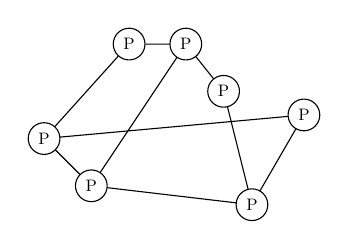
\begin{tikzpicture} [scale=0.6, transform shape]
\tikzstyle{every node}=[draw,shape=circle];
\node (v0) at (0, 2) {P};
\node (v1) at (1, 1) {P};
\node (v2) at (1.8, 4) {P};
\node (v3) at (3, 4) {P};
\node (v4) at (4.4, 0.6) {P};
\node (v5) at (3.8, 3) {P};
\node (v6) at (5.5, 2.5) {P};
\draw (v0) -- (v1)
(v0) -- (v2)
(v0) -- (v6)
(v4) -- (v5)
(v1) -- (v4)
(v2) -- (v3)
(v3) -- (v5)
(v4) -- (v6)
(v3) -- (v1);
\end{tikzpicture}
\label{p2p}
}
\caption{\cs~architecture and P2P architecture}
\end{figure}

It is widely agreed that P2P architectures outperforms \cs~in scalability, latency and robustness~\cite{Fgame, Scheating}, however, in IP networks P2P is not as popular as \cs~architectures. The factors that make P2P less desirable in the IP network are as follows. First, P2P games usually have higher bandwidth requirements than \cs~games do. In game communications a common scenario is that every player wants to exchange packets with all other players. For example, in Egal Car, every car wants to know the position of all other players, and it also want its own position to be known by others. In a P2P network this would generate an enormous amount of traffic but in a \cs~network the traffic will be alleviated because the server plays the role of an ``information center'' and each player communicate with all other players by exchanging a few packets with the server. Note that the traffic of P2P games could be alleviated by multicasting. Unfortunately, multicasting is not widely available in IP networks~\cite{Fgame} because IP is host-to-host in its nature. Second, due to the lack of an authority in P2P architectures, player authentication becomes harder while cheating becomes easier~\cite{Scheating}.

Despite being less popular than \cs~in the IP world, P2P is chosen by us for our prototype Egal Car. In NDN, P2P architectures have actually become much more desirable since NDN largely alleviates network traffic from the lower layer. NDN is intrinsically multicasting, and it guarantees that every piece of content (data) will go through a link for at most once. These makes P2P's bandwidth requirement comparable to that of \cs. Although problems with authentication and anti-cheating may still exist, the advantages of P2P architectures (smaller latency, better scalability and robustness) greatly outweigh its disadvantages. Another reason that we prefer P2P over \cs~is that the star topology of \cs~architectures (as shown in figure~\ref{cs}) cannot fully exploit the advantages of NDN's communication model. NDN reduces traffic by making use of the web cache. In P2P architectures, after a peer has obtained a certain piece of data, other peers who are close to that peer in the physical world might benefit from this fact as they may request a quick copy of the data from the previous peer's web cache instead of waiting for the same data to be sent from data publisher. The same thing will not happen in \cs~architectures, as there is no direct connection between any two clients and NDN cannot alleviate traffic for such topology.

Once the game architecture choice is made, one can start considering the other design issues of the network module such as the synchronization mechanism. To see why game architectures would affect other game design issues, one can consider the following example. In different architectures, the content of packets being transmitted would be different. In \cs~architectures, clients should always send user inputs to the server and let the server compute the result of the input. A client should never compute the result on its own because it has neither the right to compute the next game state nor the information that is sufficient for it to do so. For instance, instead of claiming ``I am three blocks away from my last position now'', a client should only tell the server ``I want to move three blocks to the north-east'' and let the server confirm its new position. On the contrary, in P2P architectures every peer has the right and the information to compute the next game state. This gives some extra freedom to each peer in deciding what to send to the other peers. A peer can choose to send out user inputs, just like a client in the \cs~architecture would, or he/she can choose to send out the result of his/her inputs and ask the other peers to update their information. The later approach is adopted in Egal Car for synchronizing each car's position information (see section~\ref{synchronization}).

%============================================================================%
\section{Synchronization}
\label{synchronization}

We propose two synchronization strategies, asset synchronization and state synchronization, that can be used as a combined mechanism by P2P MOGs over NDN. Our approach has three steps: first, identify all data that needs to be synchronized; second, classify these data as either \emph{asset} or \emph{state}; third, use asset synchronization to synchronize assets and use state synchronization to synchronize state.

%-------------------------------------------------------------------------------------------------------------------------------------%
\subsection{Namespace}
\label{namespace}

The first two steps of our approach mentioned above involves namespace design. A \emph{namespace} is a full collection of names that will be used for packet exchange during a program's execution. In our case, the namespace is consisted of all names that need to be synchronized plus names of packets that are designed for synchronization. 

We can start to construct our namespace by analyzing which classes of MOG data (objects) need to be kept in sync. According to~\cite{Upen}, a virtual world is typically made up of immutable elements (terrain) and mutable elements (players, non-player characters, mutable objects, mutable landscape). The immutable elements should be installed before game execution. Information about the mutable elements should be synchronized in real time. In Egal Car, the terrain and the track are installed while information about players (cars) are synchronized.

When the data to be synchronized is determined, the next step is to identify it as asset or state. This is based on an observation that different data ``behaves'' differently in MOGs and often have different requirements for synchronization. In Egal Car, information about player login and logout is identified as asset updates and information about a car's position and rotation is identified as state updates. Asset updates tend to be more persistent. After a player's login has been announced, this information does not need to be updated until that player logs out (or becomes disconnected). The time interval between asset updates may be measured by seconds or even minutes. State updates, however, tend to be more transient. A car's position, for example, trend to change continuously. The time interval between a state and its successor is usually measured by milliseconds. It is hard to predict when an asset update will happen or how often they will happen, as this is controlled by gamers. However, it is relatively easy to predict the frequency of state updates, as this is often defined by game applications (it is Egal Car that decides how often a position update should be published). Asset updates are about object creations and deletions while state updates are about object value changes. Once an asset's existence is known, the game application would know which state it should synchronize for the asset, since state is always a member or a child of the asset. One convenient way of identifying assets and state is to think about the object-oriented programming languages: asset updates are like constructors and destructors while state updates are like snapshots of object values.

% Namespace designing is a development process that is specific to NDN applications. A complete namespace (such as in figure~\ref{img:namespace}) of a program is a collection of all names that will be used by the Interest and Data packets being exchanged during the program's execution. Since NDN names are composed of components, we can present names as trees by treating its components as tree nodes. Names of the same application usually share the same prefix, which means a name tree can denote a large collection of names (with the shared prefix being the root node of the name tree). The namespace of an application is usually consisted of several of these name trees. Egal Car, for example, has three trees in its namespace.

\begin{figure}
\begin{center}
\begin{subfigure} [Repo Tree]
{
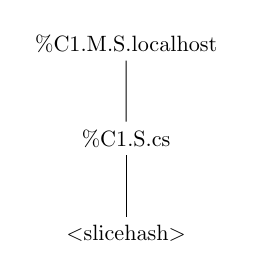
\begin{tikzpicture} [scale=0.8, transform shape]
    %\tikzstyle{every node}=[rectangle,draw]
    \node {\%C1.M.S.localhost}
        child { node {\%C1.S.cs} 
        		child{ node {$<$slicehash$>$} }
        }
    ;
\end{tikzpicture}
\label{repo}
}
\end{subfigure}
\begin{subfigure} [Network Tree]
{
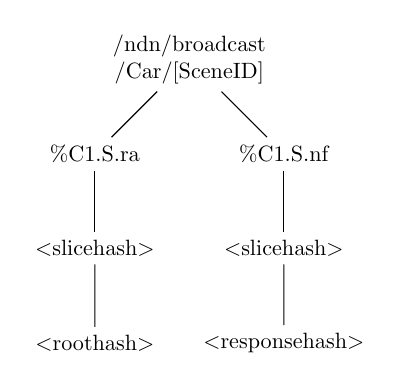
\begin{tikzpicture} [scale=0.8, transform shape]
    \tikzstyle{every node}=[align = center]
    \tikzstyle{level 1} = [sibling distance=30mm]
    \node {/ndn/broadcast \\ /Car/[SceneID]}
        child { node {\%C1.S.ra} 
        		child { node {$<$slicehash$>$} 
			child { node {$<$roothash$>$} }
		}
        }
        child { node {\%C1.S.nf}
        		child { node {$<$slicehash$>$} 
			child { node {$<$responsehash$>$} }
		}
        }
    ;
\end{tikzpicture}
\label{broadcast}
}
\end{subfigure}
\begin{subfigure} [Game Tree]
{
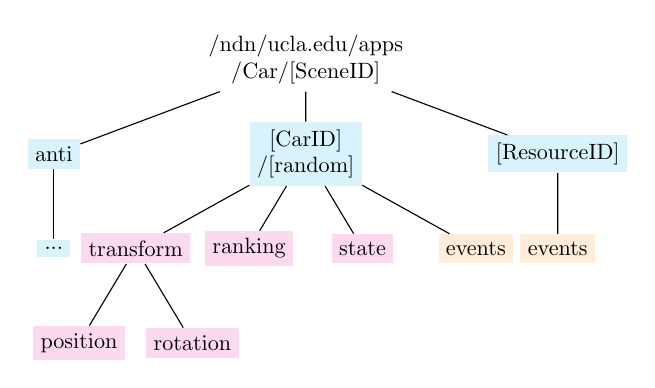
\begin{tikzpicture} [scale=0.8, transform shape]
    \tikzstyle{every node} = [align=center]
    \tikzstyle{asset} = [fill=cyan!15]
    \tikzstyle{state} = [fill=magenta!15]
    \tikzstyle{event} = [fill=orange!15]
    \tikzstyle{level 1} = [sibling distance=40mm]
    \tikzstyle{level 2} = [sibling distance=18mm]
    \node {/ndn/ucla.edu/apps \\ /Car/[SceneID]}
        child{ node [asset] {anti}
        		child { node [asset] {...}}
        }
        child { node [asset] { [CarID] \\ /[random]} 
		child { node [state] {transform} 
			child{ node [state] {position} }
			child{ node [state] {rotation} }
		}
		child { node [state] {ranking} }
		child { node [state] {state} }
		child { node [event] {events} }
        } 
         child { node [asset] {[ResourceID]}
        		child {node [event] {events}} }
    ;
\end{tikzpicture}
\label{game}
}
\end{subfigure}
\caption[Caption for LOF]{The Namespace of Egal Car\footnotemark}
\label{img:namespace}
\end{center}
\end{figure}
\footnotetext{Colors of the nodes will be explained in []. Nodes surrounded by $< >$ will be generated at run time using algorithms chosen by NDN. Nodes surrounded by $[ ]$ are variables that will be substituted with multiple values. Note that \slash~are not part of NDN names, they are for illustration purpose only.}

%-------------------------------------------------------------------------------------------------------------------------------------%
\subsection{Asset Synchronization}
\label{assetsynchronization}


%-------------------------------------------------------------------------------------------------------------------------------------%
\subsection{State Synchronization}
\label{statesynchronization}


%============================================================================%
\section{Implementation}
\label{implementation}


%============================================================================%
\section{Future Work}
\label{futurework}


%============================================================================%
\section{Conclusions}
\label{conclusions}


%============================================================================%
\bibliographystyle{plain}
\bibliography{sample}

\end{document}